\documentclass{article}

\usepackage[czech]{babel}
\usepackage[utf8]{inputenc}
\usepackage[T1]{fontenc}

\usepackage[left=2cm,text={17cm, 24cm},top=3cm, bottom=2cm]{geometry}

\usepackage{rotating}
\usepackage{graphicx} % vkládání obrázků
\usepackage{amsmath} % pokročilá sazba matematiky
% \usepackage{xcolor} % barevný text
\usepackage{siunitx} % SI jednotky
\usepackage{graphicx}
\usepackage{hyperref} % Clicable table of contents
\usepackage{color} % Color for table of contents
\usepackage{float}
\usepackage{lscape}
\usepackage{hyperref} 

\restylefloat{figure}

\hypersetup{
    colorlinks=true, %set true if you want colored links
    linktoc=all, %set to all if you want both sections and subsections linked
    linkcolor=black,  %choose some color if you want links to stand out
}

\graphicspath{ {./images} } % Include image folder

\begin{document}

% start first page
\clearpage
\begin{titlepage}
	\begin{center}
		\textsc{\LARGE Vysoké Učení Technické v Brně}\\[0.5cm]
		{\LARGE Fakulta informačních technologií }\\[4.0cm]

		\textsc{\LARGE IPP}\\[0.5cm]
		\textsc{\LARGE 2021/2022}\\[3.5cm]

		{\LARGE Projekt}\\[0.5cm]
    {\LARGE \textbf{Interpretace jazyka IPPcode22}}\\
	\end{center}

	\vfill 

	\begin{flushleft} 
		\large
		Martin Douša (xdousa00)
		\hfill
		Brno, \today
	\end{flushleft}
\end{titlepage}
\thispagestyle{empty}

\newpage
\tableofcontents

%\newpage
%\listoffigures

\newpage
% end first page

\section{Úvod}

Úkolem tohoto projektu je navrhnout a implementovat nástroje pro implementaci jazyka IPPcode22.
Parsování tohoto kódu bude implementováno v jazyce PHP a interpretace v jazyce Python.
Dále budou v jazyce PHP navrženy testy.
\section{Parser}


\subsection{Základní struktura}

Parsovací script se skládá z několika menších částí. \\
1) Deklarace regexů, lookup polí \\
2) Deklarace pomocných class (Instrukce, Argument) a funkcí \\
3) Entrypoint programu


\subsubsection{Pomocné funkce}

Úkolem pomocných funkcí je odstranit z hlavního toku programu repetitivní celky kódu a udržet ho relativně dobře čitelný.\\
Mezi takové patří hlavně funkce na kontrolu obsahu stringů pomocí regexů, sanitace vstupního stringu a jeho následné zpracování (např. odstranění nepotřebných znaků a převod speciálních znaků) a error handling.


\subsubsection{Pomocné classy}

Vlastní classy jsou využity na uskladnění a zpracování dat jednotlivých instrukcí před jejech výpisem na výstup. \\
Tato část programu není úplně nejdůležitější z pohledu funkčnosti samotného parseru, ale pomáhá s formátováním a generováním dané instrukce, což by bylo o dost náročnější bez těchto pomocných class.


\subsubsection{Entrypoint programu}

Entrypoint programu obsahuje hlavní flow programu, neboli kontrolu a zpracování argumentů, načítání vstupu a jeho předzpracování jako je odstranění komentářů, znaků nového řádku a jiných bílých znaků, parsování vstupních dat na jednotlivé komponenty instrukce, kontrolo vstupních dat a následné sestavéní instrukce do požadovaného formátu, tisknutí finální instrukce na výstup a samozřejmě také error handling.


\subsection{Argumenty programu}

Momentálně jediným podporovaným argumentem je \textbf{--help} nebo \textbf{-h} pro výpis krátkého popisu programu a jeho návratových kódu.


\subsection{Návratové hodnoty}

Pokud program projde bez chyby vrací návratovou hodnotu 0, jakékoli jiné hodnoty jsou kódy erroru.\\
1) 21 - Chybějící nebo špatný IPPcode22 header \\
2) 22 - Neznámá nebo nevalidní operace \\
3) 23 - Ostatní syntaktické errory


\subsection{Flow programu}

1) Kontrola a zpracování argumentů. \\
2) Načtení jednoho řádku ze standartního vstupu a jeho sanitace. \\
3) Header check pokud ještě nebyl nalezen. \\
4) Rozdělení načteného řádků na jednotlivé složky podle mezery nebo tabulátoru (instrukce a argumenty). \\
5) Kontrola argumentů podle zjištěné instrukce. \\
6) Tisk instrukce na výstup. \\

\section{Interpret}


\subsection{Datová struktura}

Datová struktura interpretru je složena z objektů instrukce, jejich argumentů, reprezentace datových typů, framu a proměnné a pár dalších pomocných struktur.
Objektová konstrukce je v tomto ohledu velmi výhodná z pohledu práce s daty, vzhledem ke struktuře vstupních dat, které jdou rozdělit na jednotlivé operace jež je právě možné reprezentovat jednotlivými objekty.
Bylo využito hlavně creational designu specificky builder patternu, který můžeme vidět hlavně u framu - stará se o objekty proměnných bez zásahu z venku (vytváří, přistupuje, získává), uživatel k nim běžně nepřistupuje.
Dále je tohoto paternu využito částečně u argumentů instrukce. Pokud se použije konstruktor z elementu, tak si sama vygeneruje argumenty z child elementů a provede všechny potřebné kontroly.
Ale je tu i možnost přímo předat pole argumentů. Této funkce se ale přímo nevyužívá v interpretru.

\subsubsection{Argument}
Classa pro uchování vstupních dat instrukce sládající se z indexu argumentu, typu argumentu a hodnoty.
Typ argumentu je reprezentován enum classou a patří k ní přídavné listy pro převod ze stringu na tento typ a také později na převod na typ proměnné.
Při vytváření objektu je rovnou string hodnota (hodnota obdržená z vstupních dat) převedena na odpovídající reprezentaci (například je pomocí regexu nahrazená každá escape sequence v typu string) a datový typ podle specifikovaného typu argumentu.
Rovněž jsou provedeny kontroly, jestli daná kombinace typu a hodnoty dává smysl a je vůbec možné ji převést a pokud se konverze nepovede je proces interpretace přerušen.

\subsubsection{Instrukce}
Instrukce uchovává informace nutné pro spuštění dané instrukce jako je její pořadí (používáno pouze pro sortování instrukcí v poli po načtení a vytvoření všech instrukcí),
kód instrukce a pole datových typů Argument.
Kód instrukce je reprezentován enum classou a listem pro převod stringu na tento datový typ.
Hlavní částí je class funkce from\_element, která z obdrženého elementu instrukce z XML vytvoří data samotné instrukce a zkontroluje integritu dat.
V této části se také vytváří Argumenty, testuje se jejich unikátnost a validní tag. 

\subsubsection{Proměnná}
Classa pro reprezentaci proměnných při běhu programu. Využívají se ve framech pro uložení jména, typu a hodnoty dané proměnné v framu v kterém se nachází.
Typ proměnné se liší od typu argumentu a to hlavně z důvodu, že zde je o několik typů méně (chybí například typ label a var), takže je reprezentován samostatnou enum classou a je definován list pro převod mezi těmito typy.
Proměnná se vytváří pouze pomocí jména (typ a hodnota je None - není definovaná), hodnota se zadává až po vytvoření.
Po přiřazení hodnoty funkcí je také na základě typu hodnoty zjištěn typ. Pro přístup k datovému typu a hodnotě je vytvořena samostatná funkce. Není žádoucí, aby konečný uživatel mohl ručně měnit tyto hodnoty, stejně jako jméno proměnné.

\subsubsection{Frame}
Tato datová struktura slouží pro ukládání proměnných a interakci s nimi, slouží jako prostředník místo přímého přístupu k objektům proměnné.
Obsahuje funkce pro vytvořáření, vkládání hodnot a čtení hodnot z proměnných v daném framu.


\subsection{Program flow}

\begin{figure}[H] 
	\centering
	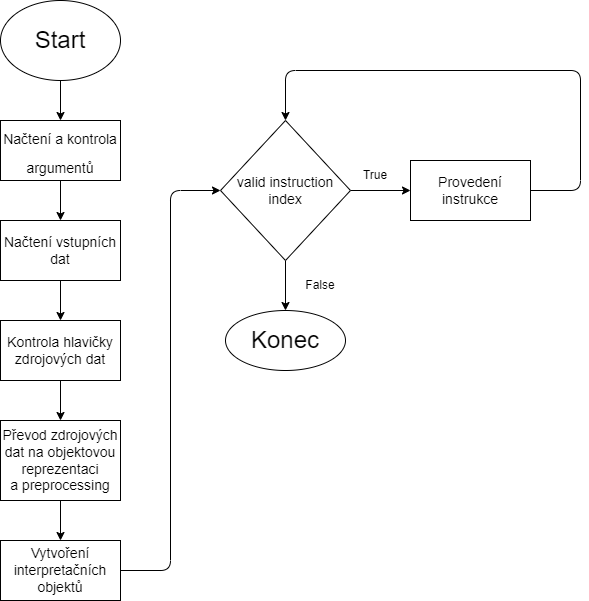
\includegraphics[scale=0.35,keepaspectratio]{intepret_diagram.png}
	\caption{Interpret flow diagram}
\end{figure}

Nejdříve dochází k načtení argumentů, kontrola jestli je zadaná kombinace validní. Parsování argumentů je implementováno pomocí knihovny argparse, která tuto operaci velmi ulehčuje a dovoluje jednoduše definovat strukturu argumentů bez nutnosti procházet ručně všemi argumentami.

Pokud byl zadán vstupní source soubor tak se rovnou celý načte a pokud specifikován není je očekáván na standartním vstupu. Dále je přes knihovnu xml je překonvertován na xml strom. Tato operace je rovnou schopná odhalit nevalidní formát vstupních dat.
Soubor vstupů je řešen jinak. Pokud je zadán, tak se celý načte a rozdělí do pole podle řádků a on demand jsou tyto jednotlivé odpovědi vraceny funkcím, které tyto data potřebují. Pokud zadaný není specifikován tak se při každém přístuúu volá funkce input a čeká se na vstup uživatele.

V dalším kroku je zkontrolována hlavička souboru (nejvyšší tag a jeho attributy) a pokud je v pořádku přechází se k převodu samotného xml stromu na objektovou reprezentaci.
Nejdříve se kontroluje typ tagu, pro případ nevalidního elementu a jsou vytvořeny jednotlivé instrukce a následně jsou uloženy do pole. V tomto kroku se rovnou kontrolují i struktury vnořených elementů a jejich attributů.
V rámci preprocessingu je potom pole instrukcí seřazeno podle order attributu a zkontrolovány duplikáty. Následně je toto pole projito znovu a je vytvořen list se jmény všech LABEL instrukcí a jejich indexů v poli instrukcí.

Dále jsou vytvořeny reprezentace pro globální frame, stack local framů a temporary frame a také call stack a data stack.

Poté už zbývá pouze procházet pole instrukcí do doby než index v tomto poli není mimo toto pole a provádět jednotlivé instrukce.

\end{document}